\documentclass{article}

\usepackage{graphicx}
\usepackage{tikz}
\usepackage{tikzsymbols}
\usetikzlibrary{calc,patterns,shapes.geometric}
\pagestyle{empty}
\usepackage[margin=0pt]{geometry}
\geometry{papersize={14in,12in}}

\def\centerarc[#1](#2)(#3:#4:#5){\draw[#1] ($(#2)+({#5*cos(#3)},{#5*sin(#3)})$) arc (#3:#4:#5);}

\begin{document}
	\begin{figure}
		\centering
		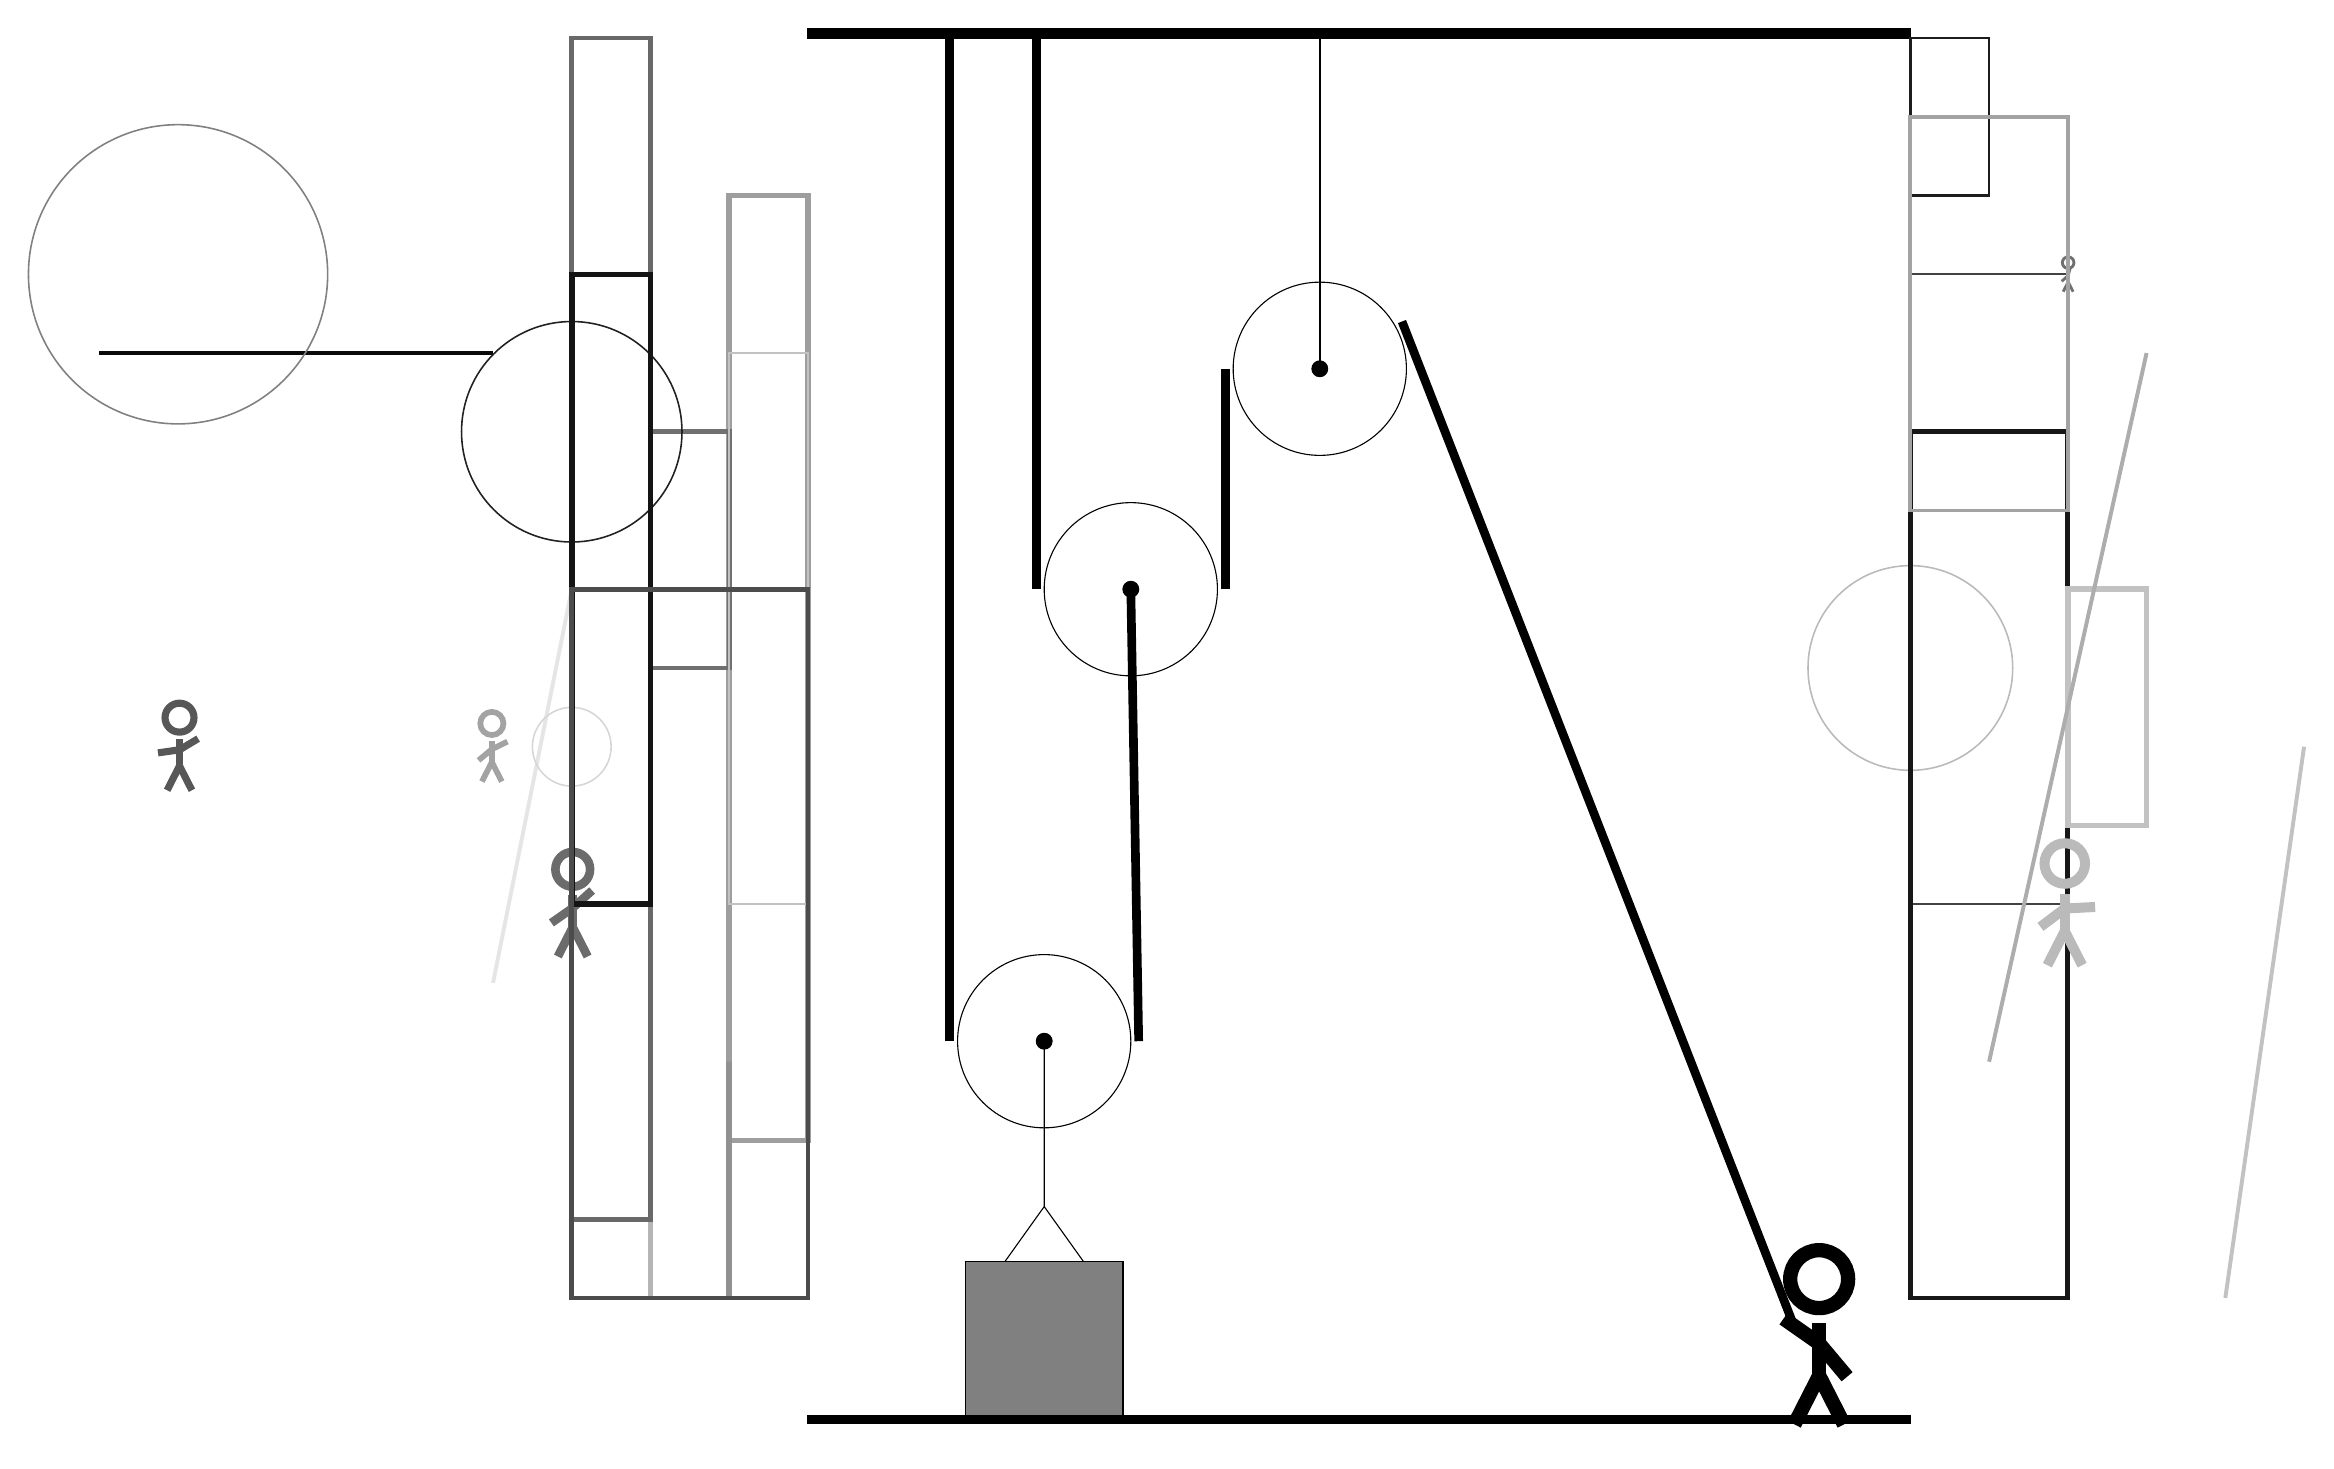
\begin{tikzpicture}
			%%%%% START %%%%%
			
			\draw[fill=black] (-2, 14) rectangle (12, 14.125);
			
			\draw (1, 1.26) circle (1.1);
			\draw[fill=black] (1, 1.26) circle (0.1);
			
			\draw (2.1, 7.0) circle (1.1);
			\draw[fill=black] (2.1, 7.0) circle (0.1);
			
			\draw (4.5, 9.8) circle (1.1);
			\draw[fill=black] (4.5, 9.8) circle (0.1);
			\draw[thick] (4.5, 9.8) -- (4.5, 14);
			
			\draw (1, 1.26) -- (1, -0.84) -- (0.5, -1.54) -- (1.5, -1.54) -- (1, -0.84);
			\draw[fill=black!50] (0, -1.54) rectangle (2, -3.54);
			
			\draw[line width=1.1mm] (-0.2, 14) -- (-0.2, 1.26);
			\centerarc[line width=1.1mm](1, 1.26)(180:360:1.2000000000000002);
			\draw[line width=1.1mm](2.2, 1.26) -- (2.1, 7.0);
			\draw[line width=1.1mm] (0.9, 14) -- (0.9, 7.0);
			\centerarc[line width=1.1mm](2.1, 7.0)(180:360:1.2000000000000002);
			\draw[line width=1.1mm](3.3, 7.0) -- (3.3, 9.8);
			\centerarc[line width=1.1mm](4.5, 9.8)(30:180:1.2000000000000002);
			\draw[line width=1.1mm] (5.544, 10.4) -- (10.5, -2.3);
			
			\draw[line width=0.7mm, color=black!38] (-2, 0) rectangle (-3, 12);
			
			\draw[line width=0.3mm, color=black!89] (13, 12) rectangle (12, 14);
			\node[line width=0.7mm, color=black!58] at (-5, 3) {\Strichmaxerl[6][35][42]};
			\draw[line width=0.7mm, color=black!29] (-4, 13) rectangle (-4, -2);
			\node[line width=0.7mm, color=black!66] at (-10, 5) {\Strichmaxerl[5][8][31]};
			\draw[line width=0.6mm, color=black!56] (-4, 6) rectangle (-3, 9);
			\draw [line width=0.2mm, color=black!27](12, 6) circle (1.3);
			\draw[line width=0.5mm, color=black!10](-5, 7) -- (-6, 2);
			\draw[line width=0.5mm, color=black!96](-6, 10) -- (-11, 10);
			\node[line width=0.2mm, color=black!56] at (14, 11) {\Strichmaxerl[2][42][75]};
			\draw [line width=0.2mm, color=black!87](-5, 9) circle (1.4);
			\draw[line width=0.3mm, color=black!74] (14, 11) rectangle (12, 3);
			\draw[line width=0.5mm, color=black!24](17, 5) -- (16, -2);
			
			\node[line width=0.6mm, color=black!36] at (-6, 5) {\Strichmaxerl[4][40][26]};
			\draw[line width=0.6mm, color=black!91] (12, -2) rectangle (14, 9);
			\draw[line width=0.7mm, color=black!43] (-3, 1) rectangle (-3, -2);
			\draw[line width=0.3mm, color=black!24] (-2, 3) rectangle (-3, 10);
			\draw [line width=0.7mm, color=black!79](16, 10) circle (0.0);
			\draw[line width=0.6mm, color=black!59] (-4, 14) rectangle (-5, -1);
			\draw [line width=0.2mm, color=black!16](-5, 5) circle (0.5);
			\draw[line width=0.5mm, color=black!36] (14, 13) rectangle (12, 8);
			
			\draw[line width=0.7mm, color=black!24] (14, 4) rectangle (15, 7);
			
			\draw[line width=0.5mm, color=black!32](13, 1) -- (15, 10);
			\draw[line width=0.7mm, color=black!92] (-4, 3) rectangle (-5, 11);
			\node[line width=0.3mm, color=black!27] at (14, 3) {\Strichmaxerl[7][37][3]};
			\draw[line width=0.6mm, color=black!70] (-2, -2) rectangle (-5, 7);
			\draw [line width=0.2mm, color=black!50](-10, 11) circle (1.9);
			
			\node at (10.8, -2.5) {\Strichmaxerl[10][-35][-50]};
			
			\draw[fill=black] (-2, -3.5) rectangle (12, -3.6);
			
			%%%%% END %%%%%
		\end{tikzpicture}
	\end{figure}	
\end{document}